\documentclass[runningheads]{llncs}

\usepackage{graphicx}
\usepackage{indentfirst}
\usepackage{hyperref}
\usepackage{algorithm}
\usepackage[export]{adjustbox}
\usepackage[noend]{algpseudocode}
\usepackage{float}
\usepackage{subfig}
\usepackage{epstopdf} %converting to PDF

\setcounter{secnumdepth}{3}
\raggedbottom

\begin{document}

% \thanks{Supported by organization x.}
\title{Parallel Genetic Algorithm for Regression}

\author{Paulo Santos \and
Maria Fidalgo
}
%\authorrunning{F. Author et al.}

\institute{Departamento de Informática da Faculdade de Ciências da Universidade de Lisboa
\email{\{fc47806,fc49034\}@alunos.fc.ul.pt}}

\maketitle

\begin{abstract}
This paper presents a series of experimental results to determine which parallel genetic algorithm is a better fit to perform linear regression. In previous research some authors have studied parallel genetic algorithms applied to different tasks or genetic algorithms for regression without focusing on its parallelization. Although the research was well conducted, some points could have been improved, like the usage of more than one test case to compare the algorithms. Nevertheless, we will show how the island model represents the better implemented approach, and which is the ideal amount of islands \textit{versus} number of cores available on the machine. Firstly, the sequential version was implemented, followed by the parallel approaches, starting by the simplest - like the ForkJoin and Phaser - and finished by developing the island model. This work is helpful for anyone who needs to apply regression to data with a lot of features.

\keywords{Parallel Genetic Programming \and Regression \and Island Model.}
\end{abstract}


%%%%%%%%%%%%%%%%%%%%%%%%%%%%%%%%%%%%%%%%%%%%%%%%%%%%%%%%%
%%%%%%%%%%%%%%%%%%%%%%%%%%%%%%%%%%%%%%%%%%%%%%%%%%%%%%%%%
\section{Introduction}

Genetic Algorithms (GAs) are metaheuristic searching algorithms where the main idea lies in following the same principles as Natural Selection and Evolution in Biology \cite{sivanandam2008genetic}. That is, the algorithms work around a \textit{population} of potential solutions for the problem, the \textit{individuals}. The population changes during the execution of the algorithm, mimicking the evolution of a real population of living beings, from generation to generation, where the fitter individuals are more likely to survive and reproduce.

The algorithm is composed by four main operations: Fitness, Crossover, Mutation and Selection. Fitness measures how good an individual is; Crossover (or sexual reproduction) generates a new solution based on two existing ones, simulating the breeding of two individuals; Mutation (or asexual reproduction) produces random changes to an individual; Selection determines how the individuals are chosen for the Crossover and Mutation \cite{langdon1995genetic}.

Due to the characteristics of the GAs, applications are often related to optimization \cite{sivanandam2008genetic}, such as the Traveling Salesman Problem \cite{grefenstette1985genetic}, classification \cite{5340522}, decision making \cite{George:2012:GAB:2345396.2345426} and prediction \cite{etemadi2009genetic}.

Prediction can be accomplished through Regression Analysis, which is the task of modeling a random variable $Y$ as a function of a vector of random variables $X$. This may be translated as the task of finding the mathematical expression best suited to explain $Y$. Regression models presuppose the existence of constants, called \textit{parameters}, that are to be estimated from the data \cite{rawlings2001applied}.

However, when using a GA for this type of problem, parameters are not we want to estimate but the whole mathematical expression. Therefore, we will be looking for the one that minimizes the error between the value provided by the model and the actual value.

In this work, we explore different parallelizations of the Genetic Algorithm for regression, using the toxicity dataset \cite{krawiec2013genetic}. We will start by introducing the algorithm and its operations in further detail. Next, we will present the several approaches studied:

\begin{itemize}
\item Sequential
\item Adaptive Sequential
\item Trivial Parallelization
\item Island Parallelization
\end{itemize}

Finally, we will demonstrate the experimental evaluation and compare with each other.

%%%%%%%%%%%%%%%%%%%%%%%%%%%%%%%%%%%%%%%%%%%%%%%%%%%%%%%%%
%%%%%%%%%%%%%%%%%%%%%%%%%%%%%%%%%%%%%%%%%%%%%%%%%%%%%%%%%
\section{Genetic Algorithm}

The implementation of a GA typically starts with a population of random individuals. Then, the population is evaluated, and reproduction operations take place \cite{whitley1994genetic}. Bellow, we present the pseudo-code for the genetic algorithm. The $AddElitesToNewPopulation$ is an optional but often used step, where a designated percentage of the best individuals are directly transfered to the new population (without any modification). This helps the algorithm to converge faster and prevents it from losing the best solutions \cite{martins2016gacuda}.

\begin{algorithmic} \small
   \State \textbf{Input}:$Max_{gen},Pop_{size},P_{cross},P_{mut},P_{reproduction}$
   \State \textbf{Output}:$S_{best}$
   \State $Population\gets InitializePopulation(Pop_{size},nodes_{func},nodes_{term})$
   \State $MeasureFitness(Population)$ \Comment{Evaluation of the population}
   \State $S_{best} \gets GetBestSolution(Population)$
   \State $Generation_{i} \gets 0$
   
   \While{$Generation_{i} \not= Max_{gen}$}
      \State $Generation_{i} \gets Generation_{i} + 1$
      \State $NewPopulation \gets \emptyset$
      \State $AddElitesToNewPopulation(Population,NewPopulation)$ \Comment{Optional}
   
      \While{$Size(NewPopulation) < Pop_{size}$}
         \State $Ind_{1}, Ind_{2} \gets SelectForCrossover(Population, P_{reproduction})$
         \State $NewGeneration \gets NewGeneration \, \cup \, Mutate(Crossover(Ind_{1},Ind_{2},P_{cross}),P_{mut})$
         \State $MeasureFitness(NewPopulation)$
      \EndWhile
      
      \State $S_{best} \gets GetBestSolution(NewPopulation)$
      \State $Population \gets NewPopulation$
   \EndWhile
   \State \textbf{return} $S_{best}$
\end{algorithmic}

%%%%%%%%%%%%%%%%%%%%%%%%%%%%%%%%%%%%%%%%%%%%%%%%%%%%%%%%%
%%%%%%%%%%%%%%%%%%%%%%%%%%%%%%%%%%%%%%%%%%%%%%%%%%%%%%%%%
\section{Approach}

\subsection{Train and Test sets}

To properly evaluate the result of each approach, the dataset was firstly shuffled and then separated  into training set (70\%) and test set (30\%). During the execution of the algorithms, only the training set was used. Afterwards, the best individual determined by the algorithm was used to calculate the error in the test set.

\subsection{Encoding}

%% types of encoding

Originally, binary encoding was used to encode the solution \cite{whitley1994genetic}. That is, an individual was represented by a vector where each entrance corresponded to some feature being true for that particular individual. Later, other types of encoding were propposed in order to represent more sophisticated types of individuals, like the value encoding, permutation encoding, and trees \cite{martins2016gacuda}. We chose the last one for our work, since our goal is to encode expressions, that can be directly mapped to Abstract Syntax Trees.

Choosing an Abstract Syntax Tree for the encoding allows us to easily generate random mathematical expressions with an immutable tree. Each node of the tree either represents a binary operator ($+,-,*,whole division$) node or a constant node, which can be a variable or value (any integer from -1000 to 1000).

The variable names were generated according to the dataset: from $x_{1}$ to $x_{n}$, where $n$ is the number of features from the dataset.

\subsection{Fitness}

The fitness function is the main responsible for the efficiency of the GA, so it must be wisely selected. In order to perform regression on the given data, it is necessary to bind the variables from the expression being evaluated and the corresponding data values. After that, the error for each data entry in computed. Bellow there is an algorithm line-up for the fitness measurement.

\begin{algorithmic}

   \State \textbf{Input}:$Data,DataOutput,Expression,Pop_{size}$
   \State \textbf{Output}:$RMSE$
   
   \State $errors \gets 0$
   \State $BindedData \gets BindDataToExpression(Data,Expression)$
   
   \For{$DataRow_{i} in BindedData$}
      \State $errors \gets errors + (DataOutput_{i} - ExpEval(BindedData_{i},Expression))^2$
   \EndFor
   
   \State $RMSE \gets \sqrt{\frac{errors}{Pop_{size}}}$
   \State \textbf{return} $RMSE$
\end{algorithmic}

Normally, the fitness function is the objective function to be maximized throughout the execution. Instead, we opted to try to minimize the fitness. That decision is based on the fact that our goal is to minimize the error. We chose to use the Rooted Mean Squared Error (RMSE) as the measure for the error between the data output and the predicted output. It is easy to see that this operation is quite heavy, and depends a lot on the size of the dataset. To alleviate the load, we used an approximate function evaluation \cite{beasley1993overview} for the first $250$ generations. The approximate approach is based on the division of the training set in parts and assign each to each generation, in turns.

\subsection{Selection}

There are many different strategies to choose the individuals for crossover and mutation, like tournament selection or rank selection.Nevertheless, we chose the most popular one, known as proportionate selection (or roulette-wheel selection). In this strategy, the probability of an individual being chosen is directly proportionate to its fitness \cite{martins2016gacuda}.

In addition, the sorting of the population is also performed, so that the first individual is the best and last the worst.

\subsection{Crossover and Mutation}

For crossover and mutation there also are multiple strategies that can be chosen. For the sake of simplicity, we opted by following the simpler approaches: one-point crossover and the uniform mutation \cite{martins2016gacuda}.

One-point crossover is accomplished by randomly selecting a point from both individuals selected and assigning the first part of the first parent to the first part of the offspring and the second part of the second parent to the second part of the offspring.

The uniform mutation consists of randomly choosing one node and changing its inner value uniformly from the available values. A constant node could have its inner content changed with a new value or variable, while a binary operator node would have its operation changed to a random one (each equally likely of being chosen).

Note that, in the context of our work, the point is one of the nodes of the tree. So, to choose the node randomly, we developed the algorithm that follows:
\begin{algorithmic}
\If {$node \, is \, Constant$}
        \State $return \,\, node$
\Else 
       \If {$index < node.left.size$} 
           \State $return \,\, findNode(node.left,\,index)$
       \ElsIf {$indice > node.left.size$}
           \State $return \,\, findNode(node.right,\,index - node.left.size - 1)$
       \Else
	 \State $return \,\, node$
       \EndIf
\EndIf
\end{algorithmic}


\subsection{Adaptive Genetic Algorithm}
The Adaptive implementation of a GA diverges from the regular implementation by not having the mutation and crossover rates fixed. Instead, the mutation and crossover rates are dynamic, and adapt depending on the progression made by each operation in the last generation \cite{adaptativeCrossOverMutation}.

The new offsprings are generated by crossing parents using an Adapted Fitness Proportionate Selection. Since new offsprings are always generated by crossing two individuals, the crossover rate will influence the probability each individual has of being chosen. This has been attained by using the absolute value of the normal probability density function, and multiplying it by the sum of a third of the amount of population with the crossover rate. The crossover rate is an integer value between \(-populationSize\) and \(populationSize\).

\[ \left |\left | \frac{1}{\sigma \sqrt{2\pi}}*e^{-\frac{(-\mu)^2}{2\sigma^2}} \right | * (popSize\,/\,3) + crossoverRate)  \right | \%  \, popSize \]	

The mutation rate controls the probability of an individual to suffer a mutation. This value is a value between 0.05 and 1.0.

Both rates are updated according to the progressions they obtained for each individual. The chosen mutation rate offset is 0.05 and the crossover rate offset is \(populationSize * 0.025\).

\begin{algorithmic}
\If {$mutationProgress < crossOverProgress$}
        \State $mutationRate := min(1.0, mutationRate + mutationOffset)$
        \State $crossoverRate := max(-popSize, crossoverRate - mutationOffset)$
\EndIf
\If {$mutationProgress > crossOverProgress$}
        \State $mutationRate := max(mutationOffset, mutationRate - mutationOffset)$
        \State $crossoverRate := min(popSize, crossoverRate + mutationOffset)$
\EndIf
\end{algorithmic}

\subsubsection{Phaser GA} \hfill \par

The Phaser approach uses phasers in order to introduce a synchronization point between all the threads running.

First of, it was decided that the \(N\) threads created should be proportional to the amount of available processors of the machine. A smaller value would not take advantage of all the processing power available, whereas a higher value would have a negative impact on the performance, since the CPU scheduler would give each one of those \(N > availableProcessors\) some share of CPU time.

Every thread is responsible for a portion of the population. In order to maintain consistency in the population over the several generations, and between different threads, it is required a synchronization point, the phaser. 

The synchronization point has been introduced before and after the transition from the old population to the new one. This is a requirement since the GA operations cannot happen until every single expression from the new population has been introduced in the current population.

Additionally, it was also introduced synchronization points before and after sorting the population. After every single individual has transitioned from the old to the new population, the thread with \(threadId := 0\) launches the \hyperref[subsubsec:parallelSort]{Parallel Population Sorting} algorithm. Once the algorithm finishes, every thread gets through the synchronization point and a new generation starts.

The phaser runs the regular GA approach to compute each individual.

\subsubsection{Island GA} \hfill \par
To improve the efficiency of the algorithm, we have also implemented an Island Model for the GA. In this model, there are several independent computations of the algorithm running on different parts of the population \cite{islandModelGA}. Consequently, synchronization points are not required.

Each island has its own portion of the population, with size  $\frac{populationSize}{amountIslands}$. Occasionally - every 20 generations - the best individual of an island is sent to a random island and waits until is picked up before the sort starts, when replaces the last (worst) individual of the population of that island.

A naive approach would be to create one island per available processor. In our approach we took into account the quantity of available processors to create and hold the computation of the islands.Therefore, it is possible to create a variable amount of islands between $1$ and the amount of available processors. If the specified amount of islands is smaller than the amount of processors then the remaining available processors will be evenly distributed through the islands - starting by the first island, allowing them to contain inner parallelization. This allows the island to split the population with the amount of threads assigned to it and compute each generation quicker.

When an island completes its computation, it redistributes the upcoming available threads with the rest of the islands, starting with the last island. This way we are able to reuse the processors once they're free.

Every island runs the regular GA approach to compute each individual.

\begin{figure}[htbp]
\centering
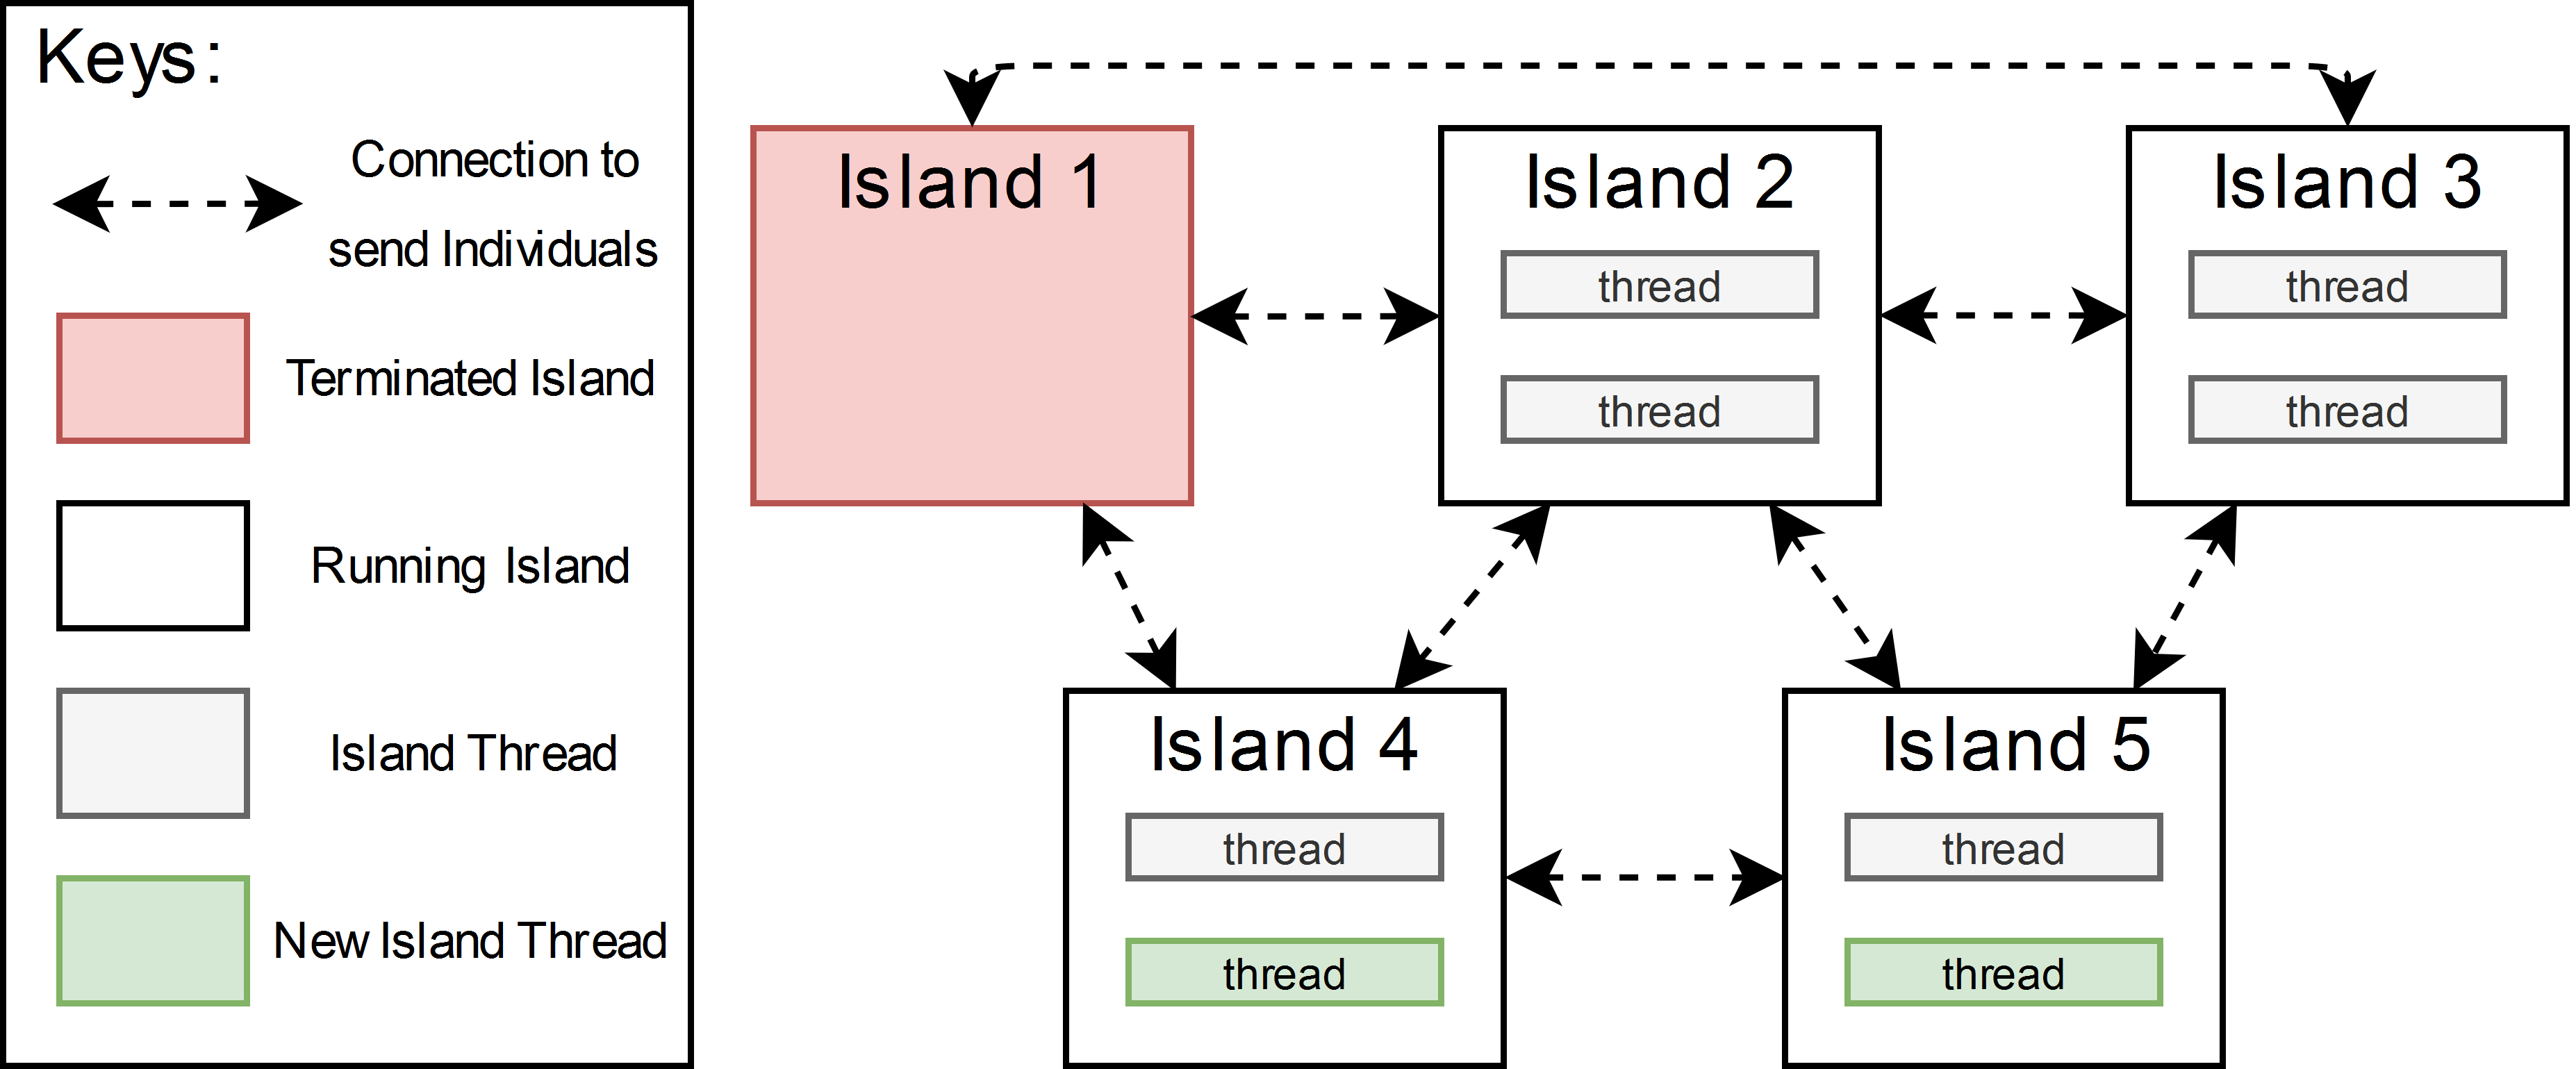
\includegraphics[width=.92\textwidth]{IslandModel.png}
\caption{Example of thread redistribution after island 1 has terminated and island 4 and island 5 create one new thread each. Settings: 8 processors, 5 islands.} \label{islandDiagram}
\end{figure}

%%%%%%%%%%%%%%%%%%%%%%%%%%%%%%%%%%%%%%%%%%%%%%%%%%%%%%%%%
%%%%%%%%%%%%%%%%%%%%%%%%%%%%%%%%%%%%%%%%%%%%%%%%%%%%%%%%%
\section{Implementation Details}

\subsection{Abstract Syntax Tree}

As mentioned above, Abstract Syntax Trees allow us to generate random mathematical expressions. Moreover, by using a Java expression builder\footnote{\href{https://www.objecthunter.net/exp4j/index.htm}{exp4j - Expression Builder from String for Java}}, it was possible to easily map values to variables of a given expression and obtain the result from it, which is useful when calculating the fitness of the tree.

\subsubsection{Parallel Population Sorting} \label{subsubsec:parallelSort} \hfill \par
Due to parallel mergesort ease of implementation and advantages of execution time \cite{analysisMergeSort}, the sorting of the population by fitness has been implemented with a parallel mergesort with linear insertion sort when the amount of population to compute is smaller than an offset of 7 .%% cita o porquê do 7
The population is split in half until the offset is reached and the insertion sort and merge algorithms' are computed.

\subsubsection{ForkJoin} \hfill \par
ForkJoin was implemented through two extensions of the Java \(RecursiveAction\) class:

\begin{itemize}
\item $GeneratePopulation$ - to generate the AST population
\item $Operations$ - to compute the GA operations (selection, crossover, mutation and fitness)
\end{itemize}

The limit from which the computation would start to be sequential was set to $2$. This allows the algorithm to divide until the end, to take advantage of the quantity of processors, and promote \textit{work stealing}.
\subsubsection{Island} \hfill \par

When an individual is sent to another island, it waits in a queue until it's turn arrives. Since this queue is accessed by all islands, it might lead to concurrency issues. To avoid that, we chose the \emph{ConcurrentLinkedQueue} to implement it.

Similarly, the redistribution of threads per islands uses a \(ConcurrentLinkedQueue<Pair<Integer, Integer>>\). When an island finishes its computation, it sends a message to another active island containing \(<islandId, \,newAmountThreads>\) so that it knows it can create new threads according to $newAmountThreads$.

Each island is implemented using the phaser approach for its inner parallelization.

%%%%%%%%%%%%%%%%%%%%%%%%%%%%%%%%%%%%%%%%%%%%%%%%%%%%%%%%%
%%%%%%%%%%%%%%%%%%%%%%%%%%%%%%%%%%%%%%%%%%%%%%%%%%%%%%%%%
\section{Evaluation}

\subsection{Experimental Setup}
The tests were made on a 24 cores machine with Intel(R) Xeon(R) CPU X5670@2.93GHz processors.

The results have been gathered by running each approach previously presented 30 times, with a population of 1.000 for 500 generations. An individual, expression tree, was able to achieve \(2^{10} + 1\) nodes when created and up to \(2^{15} + 1\) nodes after crossing with another individual. For first 250 generations the data set has been split in half and each part was tested intercalated.

\subsection{Results}
\begin{figure}[H]
\centering
\subfloat[Execution time comparison of Regular and Adaptative GA]{{ \adjincludegraphics[width=.45\textwidth, trim={50 110 15 20}, clip]{ComparisonNormalAdapTime} }}%
\qquad
\subfloat[Comparison in fitness of Regular and Adaptative GA]{{\adjincludegraphics[width=.45\textwidth, trim={50 110 25 20}, clip]{ComparisonNormalAdapFitness}}}%
\caption{Analysis of fitness and execution time performance of Regular and Adaptative Genetic Algorithms} \label{comparacaoNA}
\label{comparacaoImpl}%
\end{figure}
The Figure \ref{comparacaoNA} allows us to consider if it is worth using an Adaptative Genetic Algorithm Approach over a regular one.

Figure (a) compares the execution time of the regular and the adaptative versions. As antecipated, the Adaptative takes longer to complete the 500 generations due to having to recalculate the fitness of an individual after every crossover if it is eligible for mutation. The recalculation increased the execution time by almost 2.000 seconds, 30 minutes. The extra time could altough be justified if there ins a major growth in the fitness.

Figure (b) demonstrates an overall improvement from the Adaptative version over the Regular one. The extra 2000 seconds resulted in a progress of 100 fitness, an improvement which is not significant enough to justify the longer processing time.

\begin{figure}[H]
\centering
\adjincludegraphics[width=\textwidth, trim={85 110 25 20}, clip]{ComparisonIslands}
\caption{Comparison of the performance of the islands approach with different number of islands .} \label{comparacaoilhas}
\end{figure}

The Figure \ref{comparacaoilhas} demonstrates the execution time when using different amount of islands.

We're able to see that there is a significant difference in execution time between the islands 6,12 and islands 18,24. 

Since the islands 6 and 12 are multiple of 24, they can respectively have 4 and 2 threads for inner parallelization. Both of these islands will supposedly finish at the same time, and therefore there won't be a need of redistributing the Threads.

On the other hand the island 18, as it is not a multiple of 24, there are going to be islands with 2 threads, and islands with only 1 thread. The execution time will significantly be slower since the islands with only 1 thread represent a bottleneck in our system. However, because of the thread redistribution we are able to amortise the execution time allowing it to achieve a performance similar to the island 24 approach.

The island 24 features has an unexpected performance. Has the population is splitten evenly between the 24 islands it was expected to behave similarly to other island approaches with multiples of 24, however this is not the case. Our assumption relies on the Parallel MergeSort implemented. Each island is going to create and execute tasks to perform the sorting operation. The thread pool executor, when executed, creates N amount of threads corresponding to the amount of available proccesses. By having N amount of islands running, and each one of them creates a pool of 24 threads to compute the sorting algorithm, by the end we'll have $N*N$ threads. The CPU will have to schedule all of these threads, which implies an issue in terms of performance.

\begin{figure}[H]
\centering
\subfloat[Execution time comparison of linear implementation versus parallel implementations]{{ \adjincludegraphics[width=.75\textwidth, trim={90 110 15 20}, clip]{ComparisonWithLinear} }}%
\qquad
\subfloat[Execution time comparison of the parallel implementations]{{\adjincludegraphics[width=.75\textwidth, trim={90 110 25 20}, clip]{ComparisonNoLinear}}}%
\caption{Comparison in execution time of the different implemented approaches.} \label{comparacaolinear}
\label{comparacaoImpl}%
\end{figure}

The Figure \ref{comparacaoImpl} (a) represents the difference between the linear approach and the speedup obtained from the parallel aproaches. The linear approach required up to 50x the time from the best parallel approach implemented to accomplish the computation.

On the Figure Figure \ref{comparacaoImpl} (b) we have a comparison of the execution time between the best island approach and the ForkJoin and Phaser approach.

Through the data gathered we're able to see that the island approach takes on average less than 80 seconds than the Phaser approach. If we recall the Phaser implementation, it contains synchronization points, for example, before and after sorting the population. By having 24 inner threads, in every generation, every thread is required to wait for others in order to advance. This situation has an impact in performance, which is clearly visible on the Phaser violion plot. On the other hand, has the island6 only contains 4 inner threads, the amount of waiting required for each other is far less than waiting for 24 inner threads.

The island approach in comparison with the ForkJoin approach demonstrates a difference on average of 40 seconds probably due to the costs of creating tasks every generation. Even though these costs are low, when multiplied by the population size and amount of generations, it may have an impact on execution time later on.


%\begin{figure}[htbp]
%\centering
%\adjincludegraphics[width=\textwidth, trim={35 110 25 20}, clip]{ComparisonPopulation}
%\caption{Comparison of the behavior when varying the population size.} \label{comparacaopopulacao}
%\end{figure}

\begin{figure}[H]
\centering
\adjincludegraphics[width=\textwidth, trim={90 110 25 20}, clip]{ComparisonFitness}
\caption{Comparison of the fitness achieved for each approach.} \label{comparacaofitness}
\end{figure}

The Figure \ref{comparacaofitness} addresses the differences between the approaches implemented.

Due to the nature of separability and independence of individuals between islands \cite{islandModelGA} we can point the small improvement of fitness in the Island approach.
The remaining parallel approaches have obtained a fitness higher than the linear approach. This may have happened due to the random nature of the generated mathematical expressions.

%\begin{figure}[H]
%\centering
%\adjincludegraphics[width=\textwidth, trim={70 110 25 20}, clip]{ComparisonErrors}
%\caption{Comparison between the approaches when evaluating its best individual in the test set.} \label{comparacaoerros}
%\end{figure}

\begin{figure}[H]
\centering
\adjincludegraphics[width=.85\textwidth, trim={120 70 100 50}, clip]{GraficoTodos.pdf}
\caption{Comparison of fitness evolution through time on the parallel approaches} \label{comparacaoLinhas}
\end{figure}

The Figure \ref{comparacaoLinhas} above shows how the fitness values improve over team for each approach.

During the first 250 generations the training set is splitten in half and tested in alternate. Therefore a mathematical expression which was the best individual last generation may not be as good in the current one influencing the overall fitness by arising it. In the figure, the ForkJoin and Phaser approaches both have 2 lines in the beginning which represent the data split. The island approacha didn't have much difference between generations and therefore it only contains one line.

Through the results we are able to evaluate that the island approach achieves a better fitness earlier than the other parallel approaches.

\subsection{Discussion}

We could also conclude that even though the Adaptative Genetic Algorithm allows an overall improvement over the evaluated fitness, it drawbacks, such as the execution time, which makes it an ineligible genetic algorithm approach in our case.

According to the results we are able to conclude that the best approach was the Island. Inside of the Island approach the right amount of islands according to results were 6 Islands, a quarter of the amount of available processors. This allows inner parallelization to happen without to many synchronization points while allowing a higher population diversity.

The parallelization of the merge-sort was relevant on the Island 24 Approach as it influenced the execution time since multiple parallel work was occuring at the same time. Due to the great amount of parallel work the CPU would have to schedule this work having an impact on the processing time.

The parallelization with Phasers with a low amount of population and high amount available processors represents a problem in terms of synchronization problems. With a low amount of population the costs of synchronization between threads with phasers is high enough to have an impact on execution time. Therefore for a smaller population size a ForkJoin approach seems more reasnoable.

%%%%%%%%%%%%%%%%%%%%%%%%%%%%%%%%%%%%%%%%%%%%%%%%%%%%%%%%%
%%%%%%%%%%%%%%%%%%%%%%%%%%%%%%%%%%%%%%%%%%%%%%%%%%%%%%%%%
\section{Related Work}

Several implementations of the genetic algorithm were made throughout the years. We will shortly talk about two implementations and how they fit in the scope of our work.

Dominic and Willis  \cite{GPTIPS} developed a MATLAB toolbox, GPTIPS, which is able to perform regression through genetic programming. The main difference between their approach and  ours is that they do not explore the parallelism of the algorithm, focusing on the usability of the toolbox. Moreover, they chose to include nonlinear operators, that we decided to leave out. Our work is, therefore, important to whom intends to develop a fast approach of the genetic classifier. Additionally, GPTIPS requires the purchase of a payed software (MATLAB), available to a less broader population.

Jenetics \cite{jenetics} is another genetic programming implementation. It is a Java library designed to abstract different concepts within the genetic programming panorama, such as Gene, Genotype and Chromosome, allowing it to serve a vast spectrum of domains. This library implements the Java Stream Interface and provides ForkJoin Parallelization. This is, therefore, a generic purpose implementation for genetic algorithm. On the other hand, in our work we provided a study of genetic programming specific for regression, where other parallelization techniques were able to achieve better results than ForkJoin, like the Island Models.

%%%%%%%%%%%%%%%%%%%%%%%%%%%%%%%%%%%%%%%%%%%%%%%%%%%%%%%%%
%%%%%%%%%%%%%%%%%%%%%%%%%%%%%%%%%%%%%%%%%%%%%%%%%%%%%%%%%
\section{Conclusions}

To summarize, the Island model is with no doubt  the best algorithm to use when applying regression to a dataset with a considerable amount of features - like the toxicity dataset used for this work. Moreover, it is essential to take into consideration the number of cores when choosing the number of islands for the model, since it affect greatly the execution time.

In the future, other models could be also considered, such as the dynamic island model \cite{meng2017dynamic}, that shows a different type of interaction between different island individuals. Furthermore, the approach followed to compare the different algorithms should involve the benchmarks for more than a dataset, to have more confidence on the results. These are some improvements or ideas that could have been explored if time was not a constraint.

Finally, it would be interesting to determine if the rates for crossover and mutation, calculated by a GA, would  improve the error of the final solution.

%%%%%%%%%%%%%%%%%%%%%%%%%%%%%%%%%%%%%%%%%%%%%%%%%%%%%%%%%
%%%%%%%%%%%%%%%%%%%%%%%%%%%%%%%%%%%%%%%%%%%%%%%%%%%%%%%%%
\section*{Acknowledgements}

As for the Abstract Syntax Tree, Paulo Santos implemented the structure of the tree, the crossOver method, toString and comparator for the evaluation of the mathematical expression. Maria Fidalgo was responsible for randomly generating the tree and mutation of a tree node.

Both Authors participated on the implementation of the Sequential Version of the classifier and the LoadData class to load the data set.

Maria Fidalgo was responsible for the TestsetHandler where the evaluation of the test set with the best individual occurs.

Paulo Santos implemented the Parallel MergeSort Algorithm and the Adaptative Genetic Algorithm.

Maria Fidalgo implemented the ForkJoin Approach. Paulo Santos implemented the Phaser Approach.

Both Authors participated in the creation of the Islands Approach.

Both Authors wrote this paper, with Maria Fidalgo focusing on Abstract, Introduction, Genetic Algorithm, Related Work and Conclusions while Paulo Santos focused more on Implementation, Discussion and Results. Both participated on the Approach.

Each author spent around 50 hours on this project.

\bibliographystyle{splncs04}
\bibliography{bibliography}

\end{document}
